\section{Radar}
	Considere:
	\begin{align}
		y_{a} = ax_{a}(t-t_{d}) + v_{a}(t) \\
		x[n] = x_{a}[nT_{s}] \\
		y[n] = ax_{a}[nT_{s}] + v_{a}[nT_{s}] = ax[n-D] + v[n]
	\end{align}
	\subsection{Obtención del retardo D}
		Sea la correlación cruzada:
		\begin{equation}
			r_{xy}[n] = \sum_{k=-\infty}^{\infty} x[k] \cdot y[n+k] = x[n]*y[n]
		\end{equation}
		
		Usando esta definición se puede obtener que la máxima correlación se obtendrá cuando las señales sean lo más parecidas posibles dado que la multiplicación será máxima. Aplicando esto a las señales del sistema dado:
		\begin{equation}
			r_{yx}[n] = \sum_{k=-\infty}^{\infty} y[n] \cdot x[n-k]  \equiv \sum_{k=-\infty}^{\infty} \left( ax[n-D] + v[n] \right)  \cdot x[n-k] 
		\end{equation}
		
		El valor máximo para la correlación ocurrirá cuando $k = D$. De esta forma, buscando cuando ocurre el máximo se puede estimar el valor del desfase entre las señales. Consideremos la correlación de la señal que vuelve al radar sobre sí misma:
		\begin{equation}
			r_{yy}[n] = \sum_{k=-\infty}^{\infty} y[n] \cdot y[n-k]  \equiv \sum_{k=-\infty}^{\infty} \left( ax[n-D] + v[n] \right)  \cdot \left( ax[n-D-k] + v[n-k] \right)
		\end{equation}
		
		Para este caso, no se puede extraer información acerca del retraso D, dado que el máximo valor se obtendrá para k = 0.
	\subsection{Simulación con parámetros a = 0.9 , D= 20}
		\begin{figure}[H]
			\center
			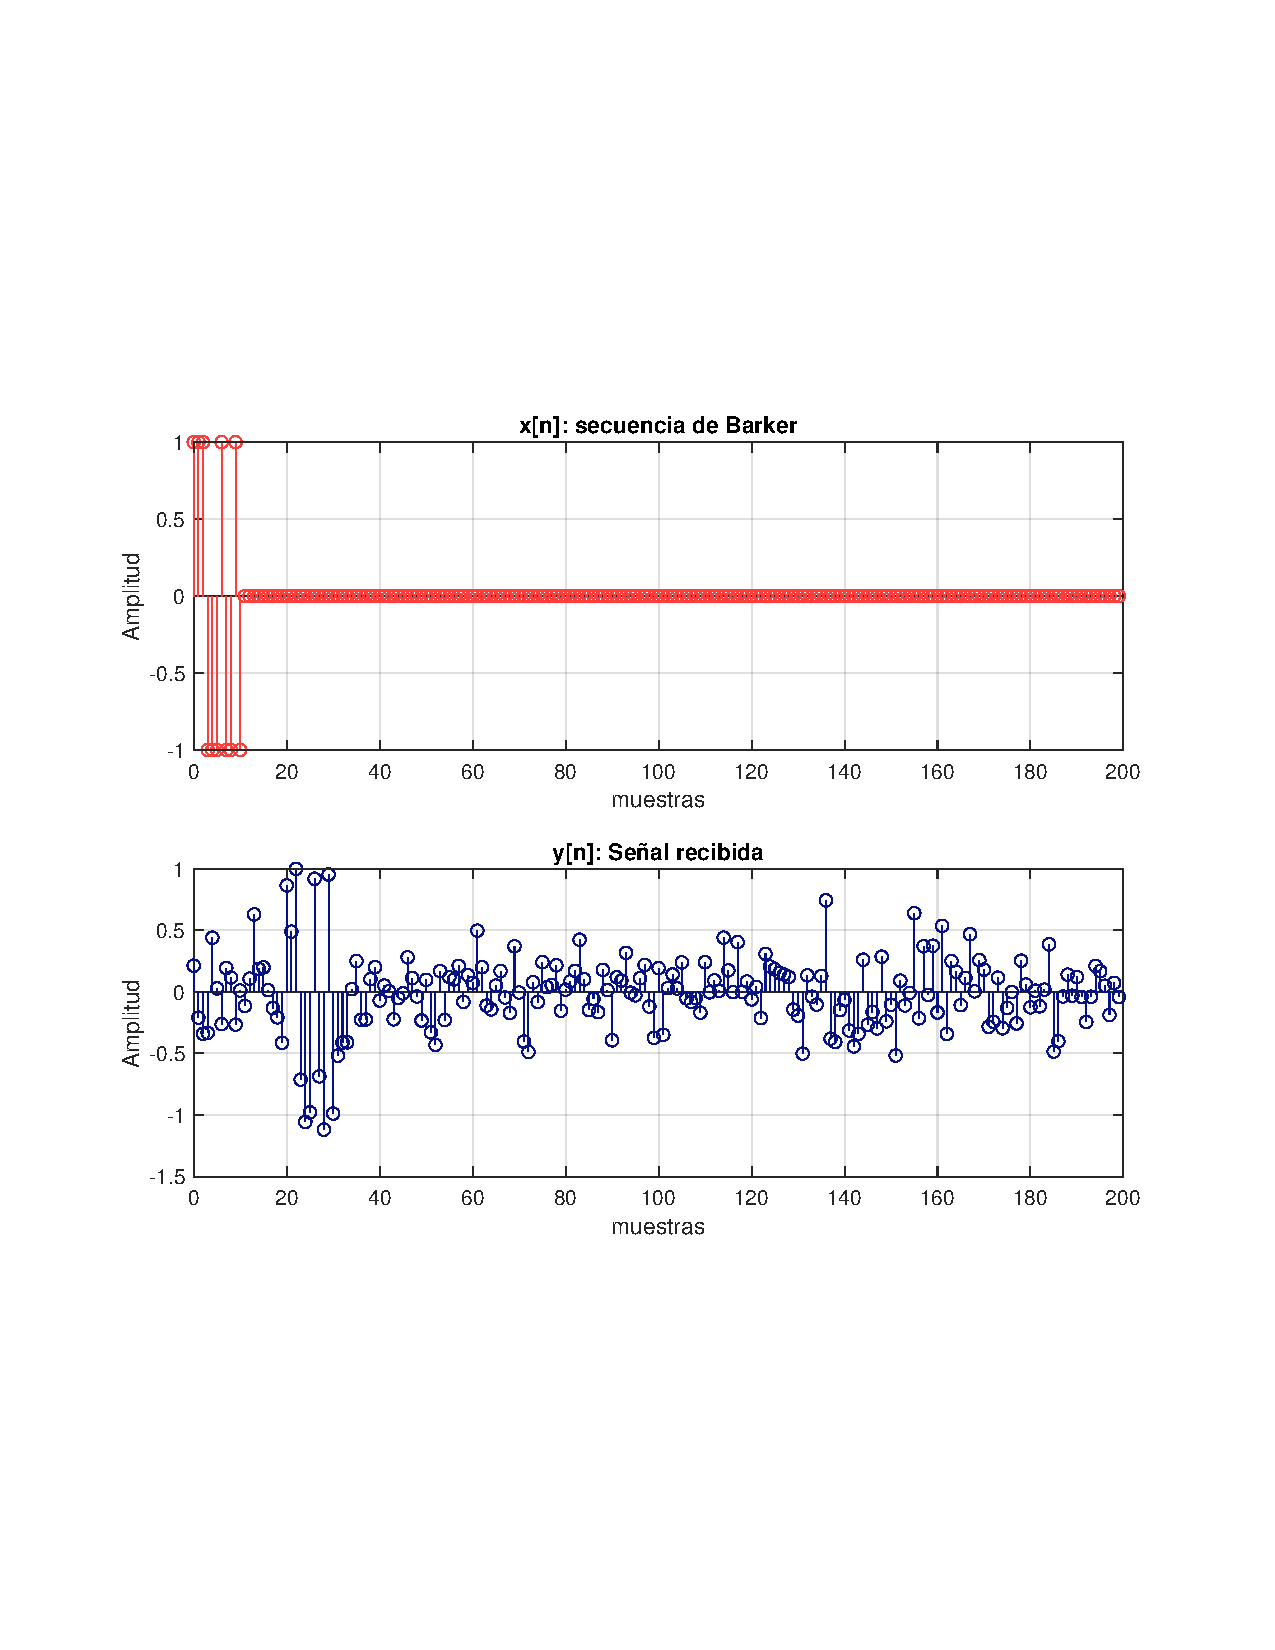
\includegraphics[width=0.6\textwidth,clip, trim = {2cm 7.0cm 2.2cm 7.0cm}]{../imgs/4_radar_b.pdf}
			\caption{Simulación de la situación}
			\label{fig:radar_b_sim}
		\end{figure}
		
		Pese al ruido, es posible encontrar la secuencia de barker reflejada.
		
	\subsection{Correlación ryy e ryx de la señal anterior}
		\begin{figure}[H]
			\center
			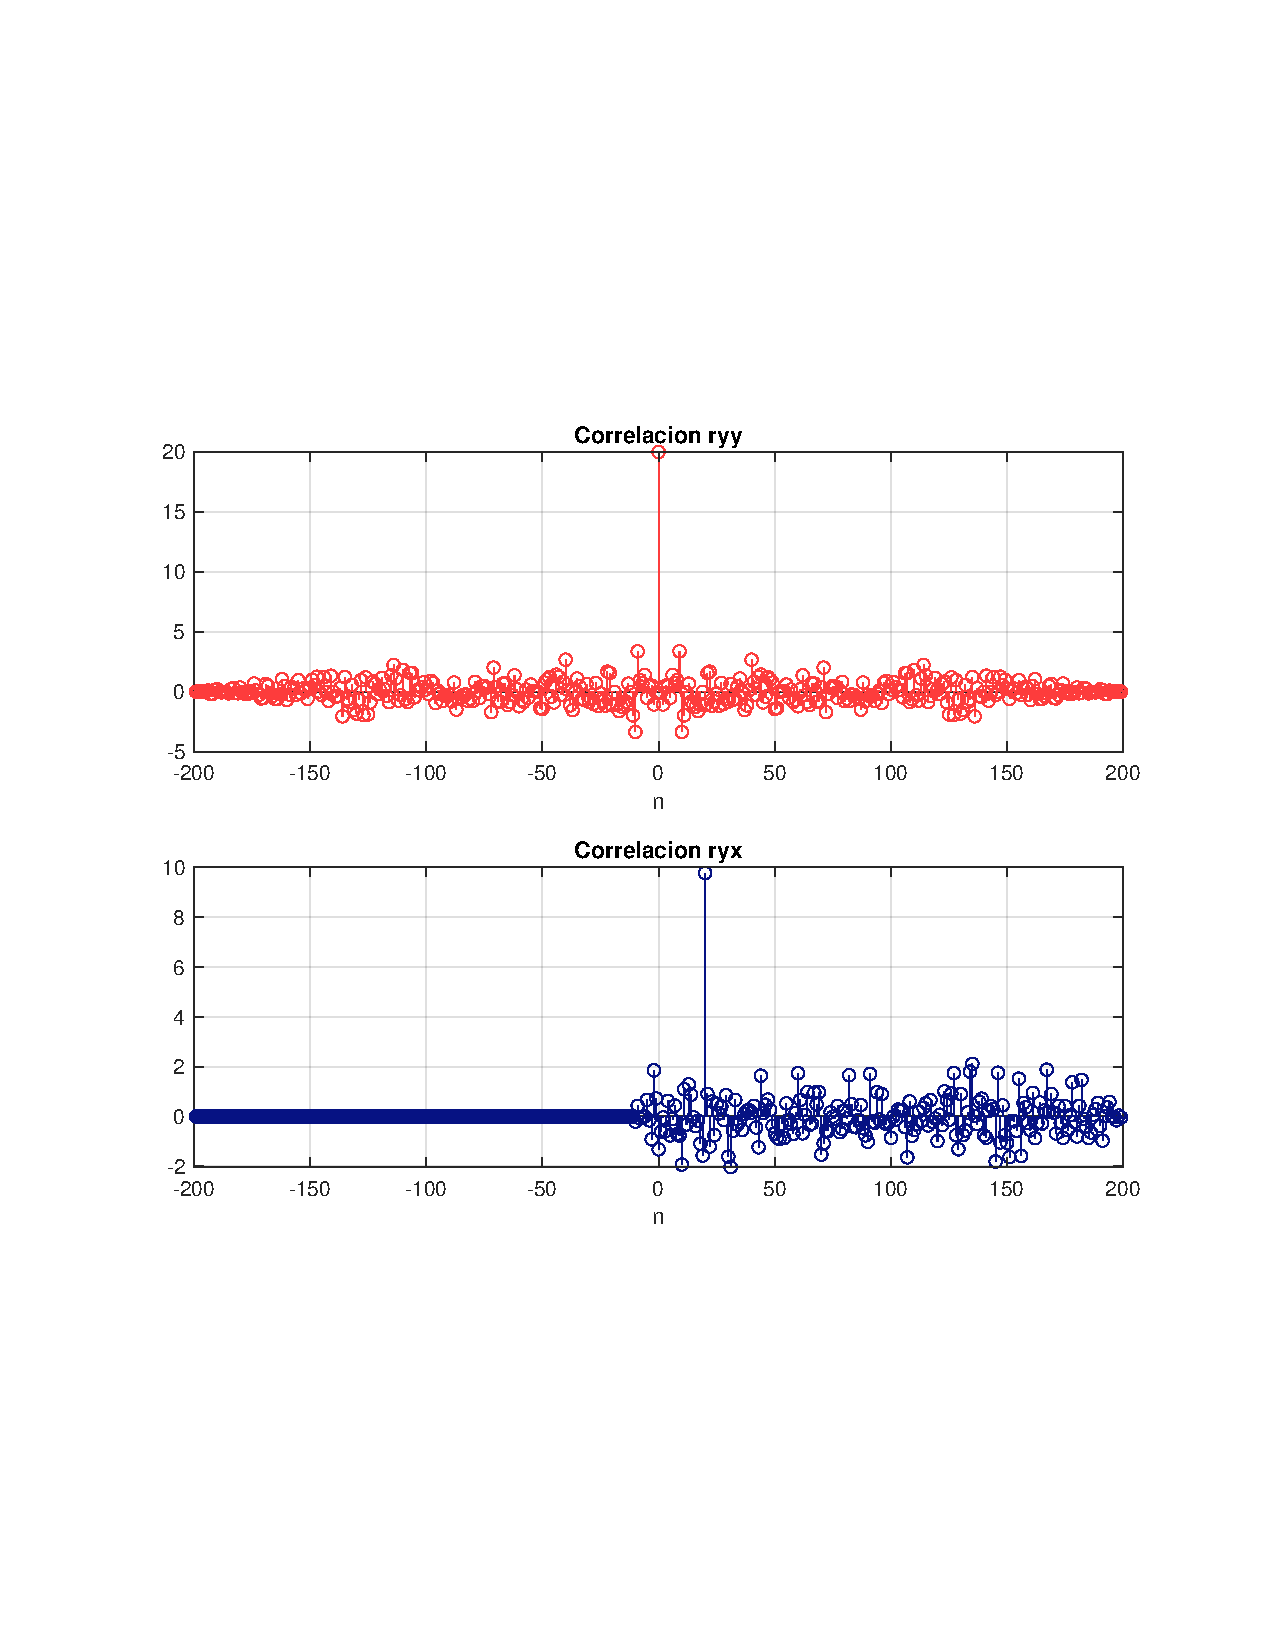
\includegraphics[width=0.6\textwidth,clip, trim = {2cm 7.0cm 2.2cm 7.0cm}]{../imgs/4_radar_c.pdf}
			\caption{Correlación ryy e ryx de la situación anterior}
			\label{fig:radar_c_ryy_ryx}
		\end{figure}
		
		A partir de estos gráficos es posible confirmar las predicciones hechas al momento de buscar una forma de encontrar el retardo. La correlación cruzada ryx, permite encontrar el retardo D, al observar el peak que esta presenta en n = 20. En cambio la correlación ryy no permite obtener el valor del retardo, dado que el peak ocurre en n = 0. Obteniendo el valor de SNR\footnote{Utilizando el comando correspondiente en Matlab}, se obtiene que la señal y[n] y el ruido están en una relación de 2.472 \textit{dB}. 
		
	 \subsection{Simulación con nuevos parámetros de ruido}
	 	\subsubsection{$\sigma^{2} = 0.1$}
	 		\begin{figure}[H]
			\center
			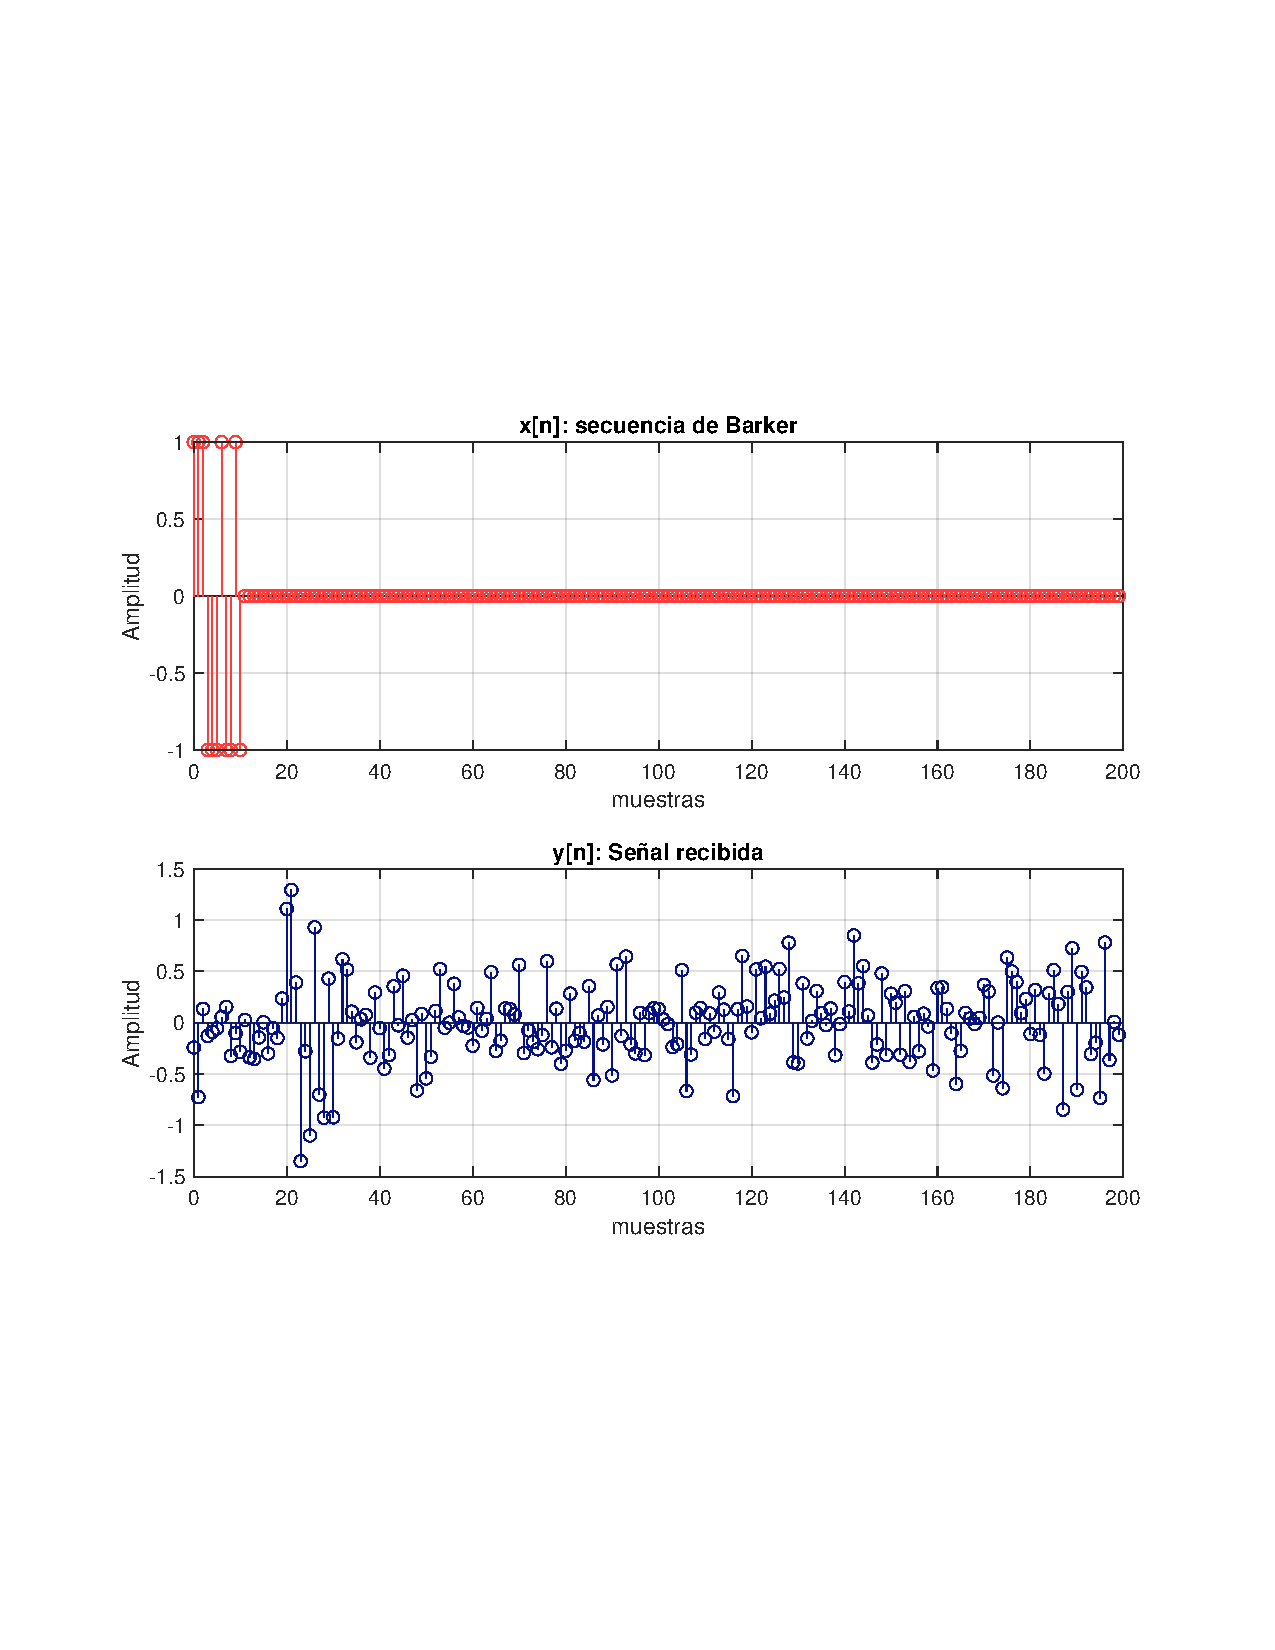
\includegraphics[width=0.6\textwidth,clip, trim = {2cm 7.0cm 2.2cm 7.0cm}]{../imgs/4_radar_d_0_1_signal.pdf}
			\caption{Simulación de la situación}
			\label{fig:radar_d_0_1_sim}
			\end{figure}	
			
			\begin{figure}[H]
			\center
			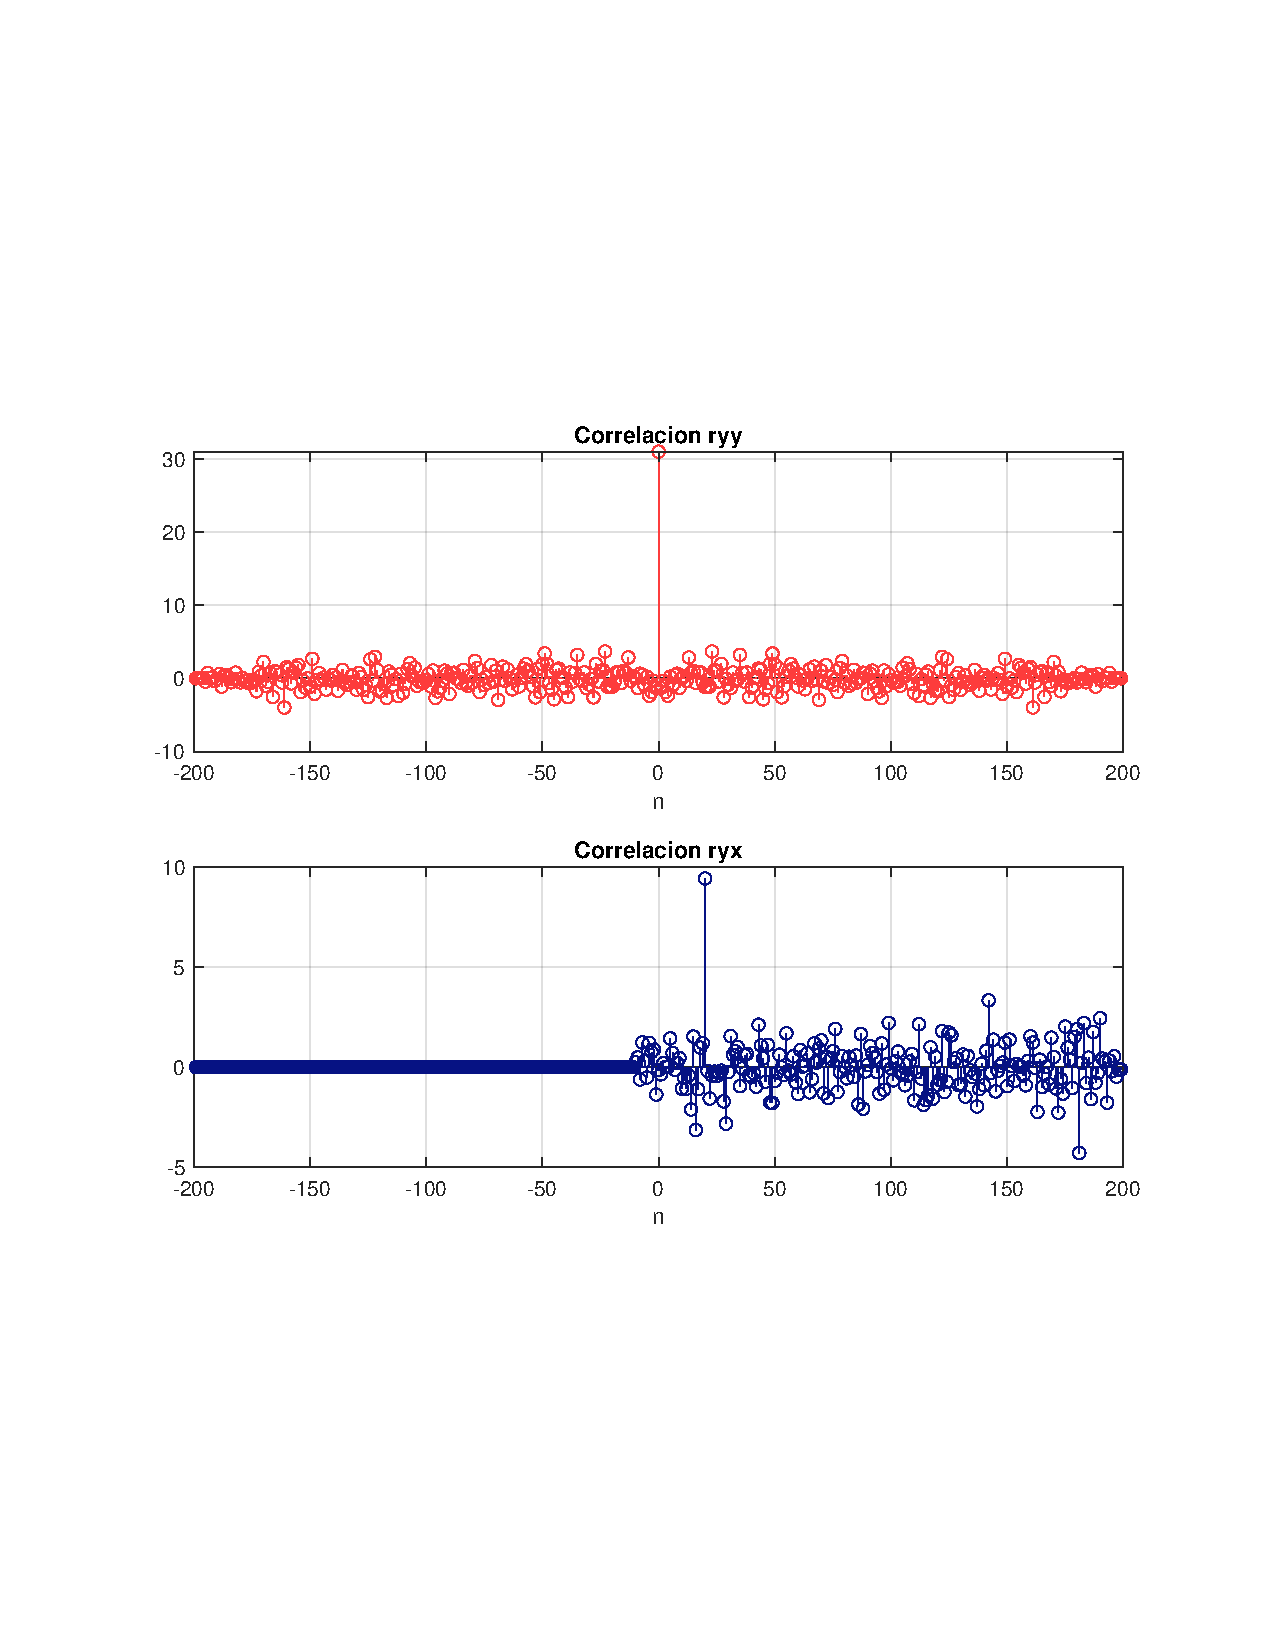
\includegraphics[width=0.6\textwidth,clip, trim = {2cm 7.0cm 2.2cm 7.0cm}]{../imgs/4_radar_d_0_1_corre.pdf}
			\caption{Correlación ryy e ryx de la situación anterior}
			\label{fig:radar_d_0_1_corre}
		\end{figure}
		
		Para este nuevo caso, se tiene un SNR de 1.30 \textit{dB}, lo que implica que al aumentar la variancia la señal se vuelve más suceptible al ruido. Sin embargo, la estimación del retraso sigue otorgando el mismo valor a partir de la correlación D = 20.
		
		\subsubsection{$\sigma^{2} = 1$}
	 		\begin{figure}[H]
			\center
			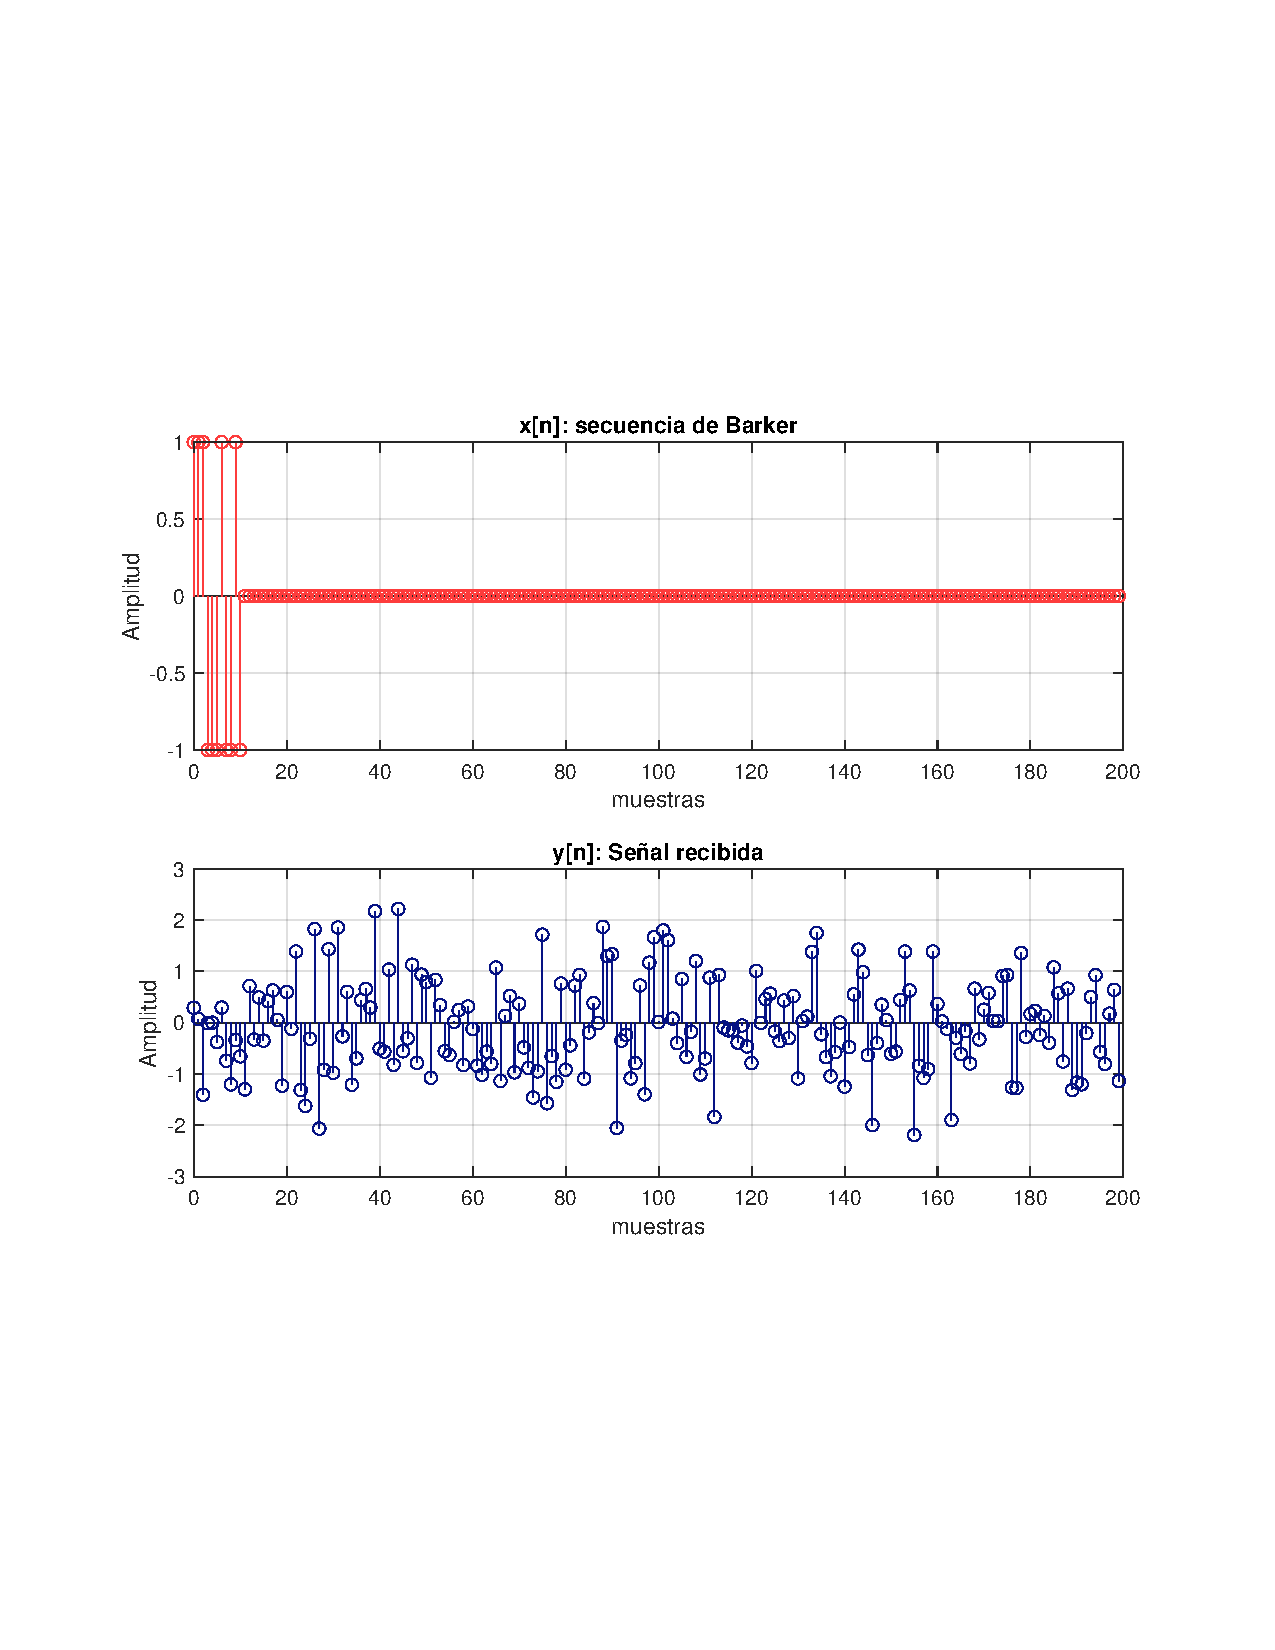
\includegraphics[width=0.6\textwidth,clip, trim = {2cm 7.0cm 2.2cm 7.0cm}]{../imgs/4_radar_d_1_signal.pdf}
			\caption{Simulación de la situación}
			\label{fig:radar_d_1_sim}
			\end{figure}	
			
			\begin{figure}[H]
			\center
			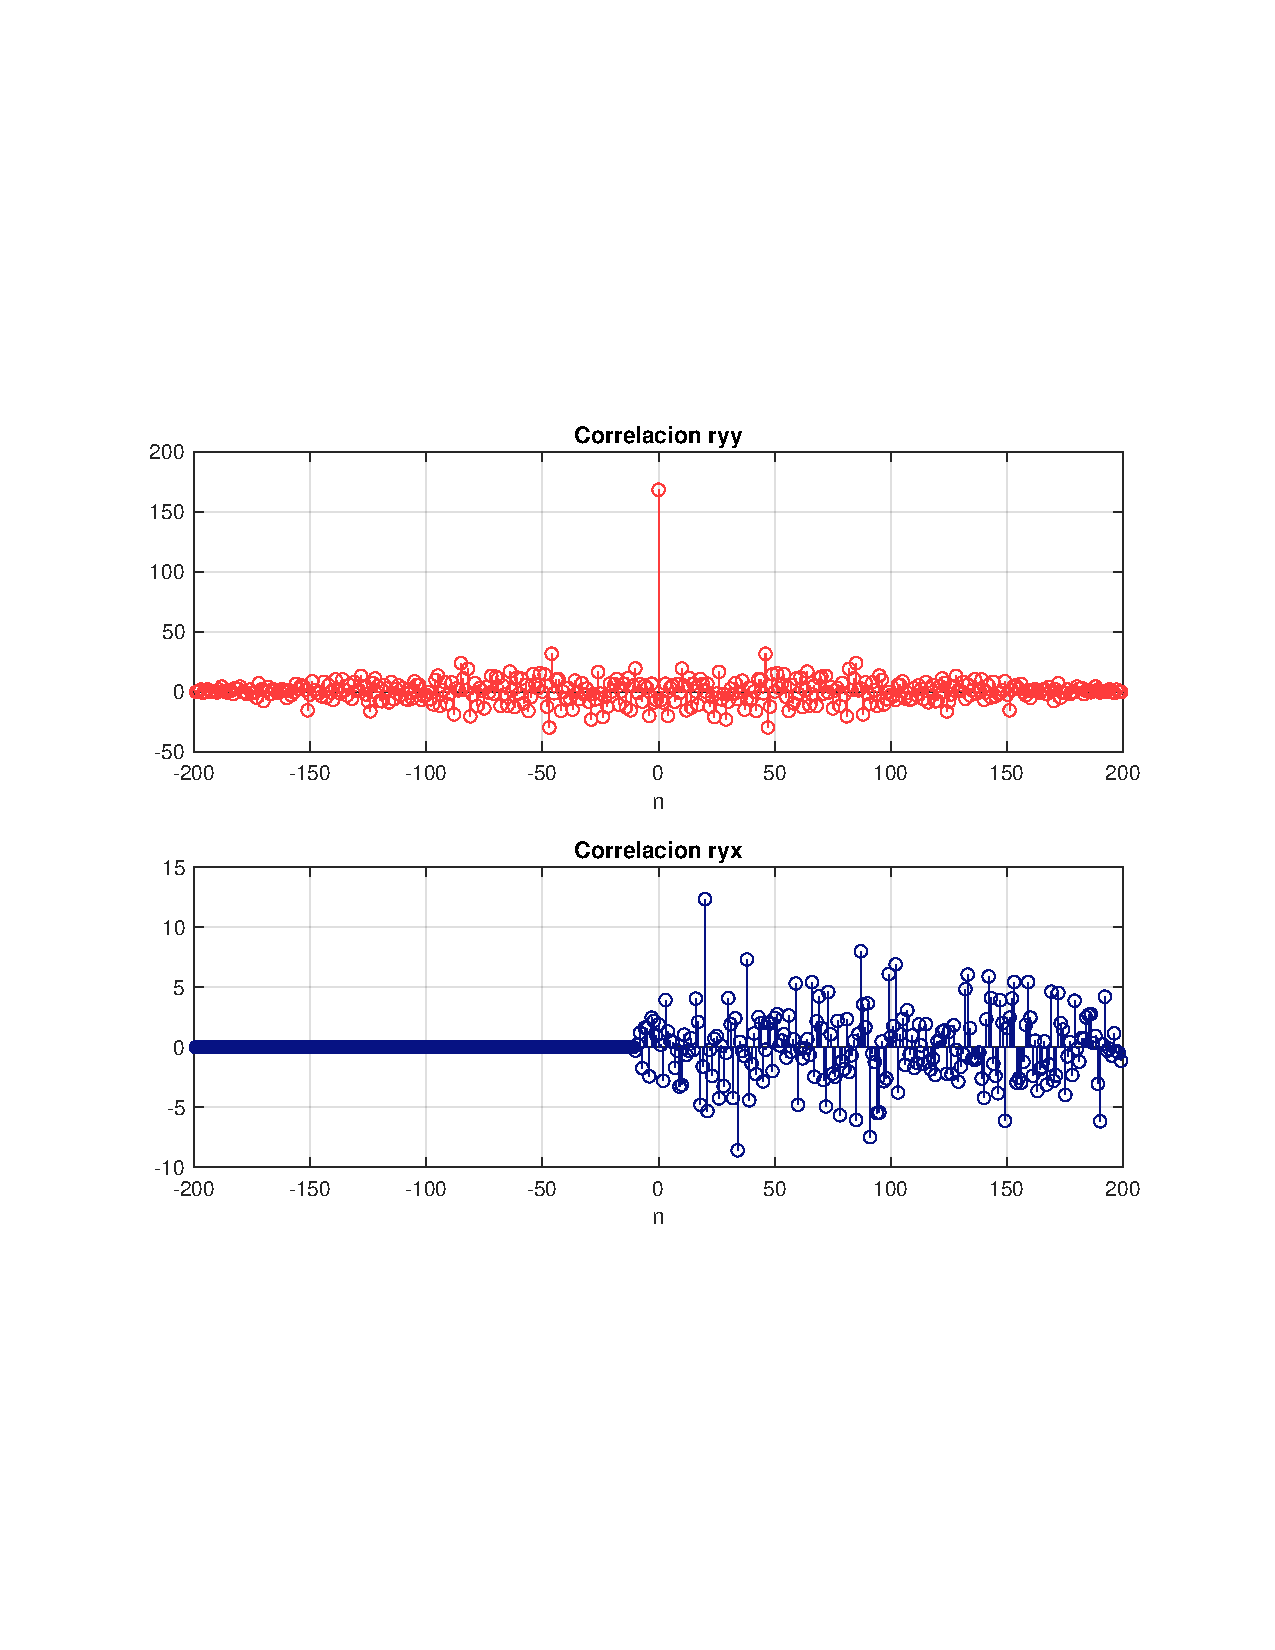
\includegraphics[width=0.6\textwidth,clip, trim = {2cm 7.0cm 2.2cm 7.0cm}]{../imgs/4_radar_d_1_corre.pdf}
			\caption{Correlación ryy e ryx de la situación anterior}
			\label{fig:radar_d_1_corre}
		\end{figure}
		
		Siguiendo con la misma tónica que el punto anterior, ahora con un SNR = 0.357 \textit{dB}, aun es posible determinar el retardo de la señal a partir del peak de la correlación. Sin embargo, ahora empiezan a aparecer peaks secundarios importantes que hacen especular que si se sigue aumentando, esta estimación podría empezar a ser imprecisa.
		
		\subsection{Simulación con 10 secuencias de Barker}
			\begin{figure}[H]
			\center
			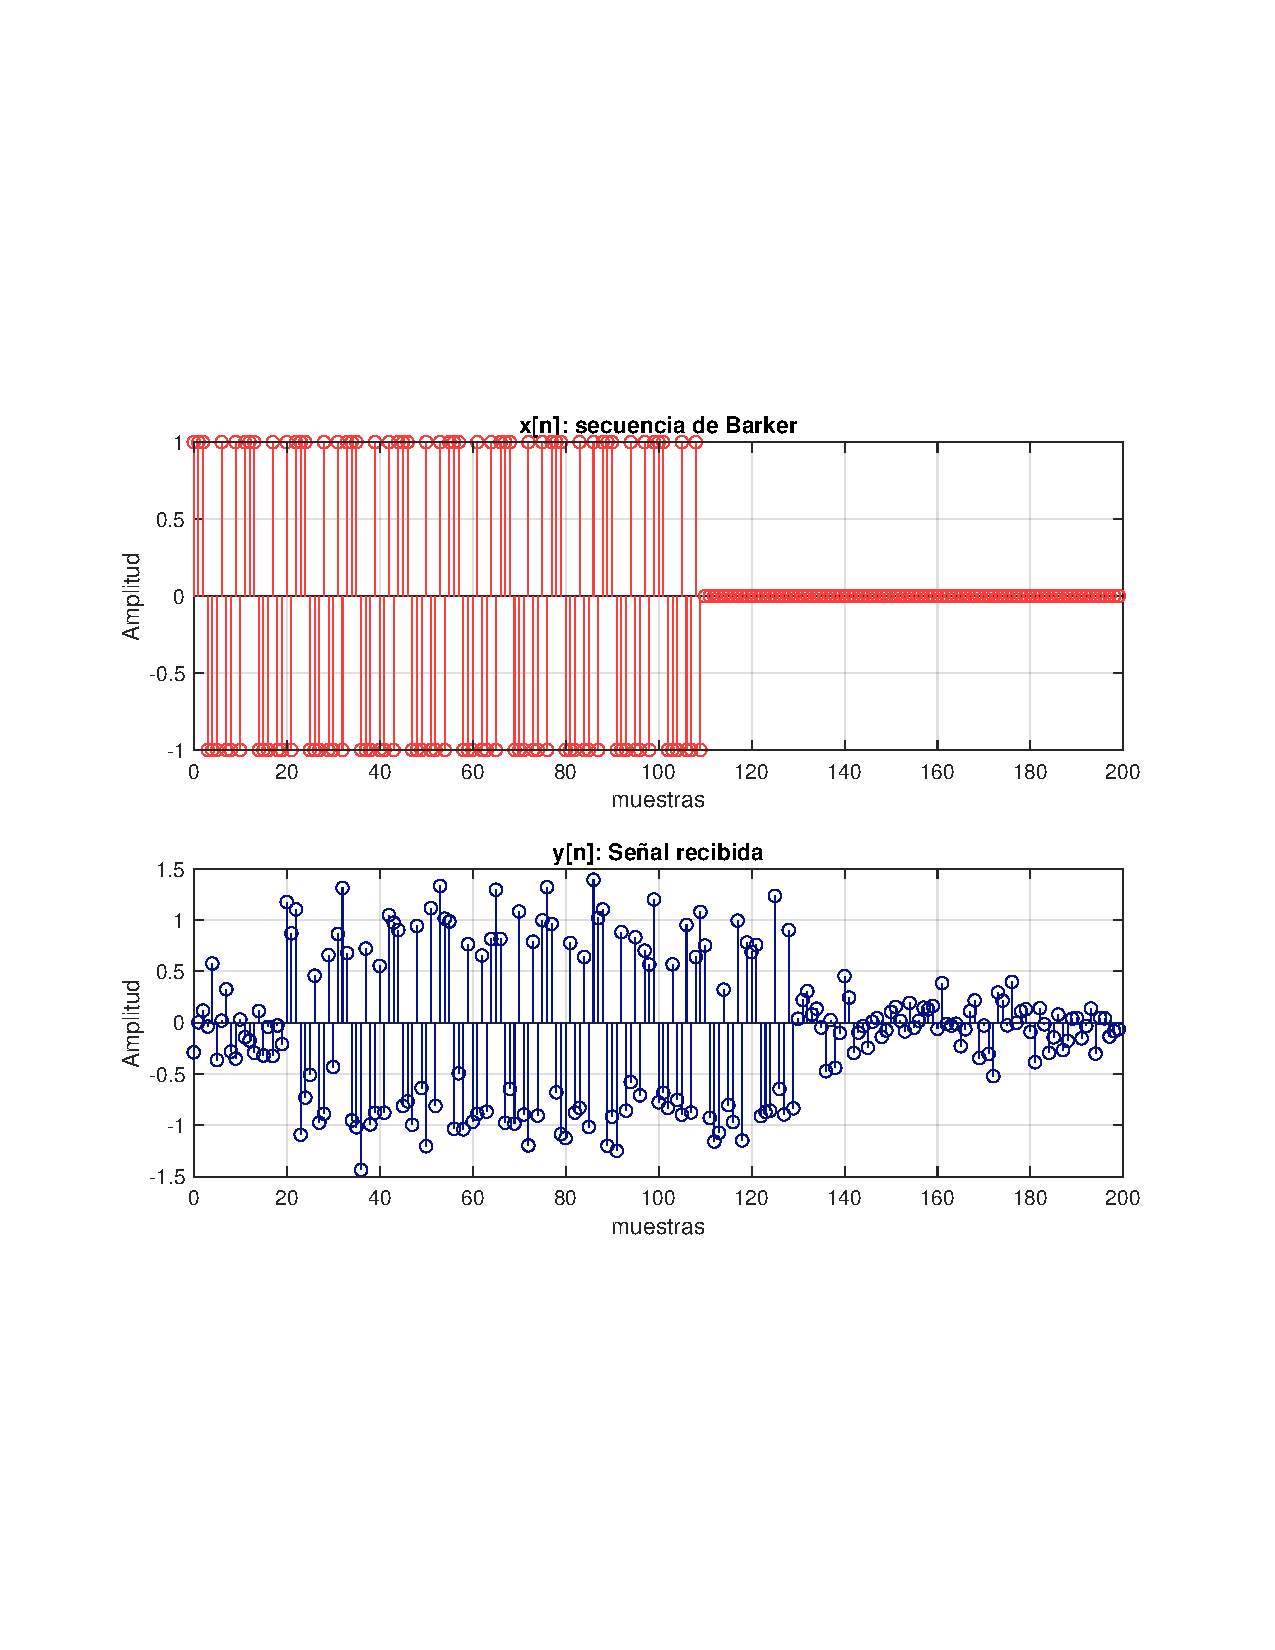
\includegraphics[width=0.6\textwidth,clip, trim = {2cm 7.0cm 2.2cm 7.0cm}]{../imgs/4_radar_e_signal.pdf}
			\caption{Simulación de la situación}
			\label{fig:radar_e_signal}
		\end{figure}
		
		\begin{figure}[H]
			\center
			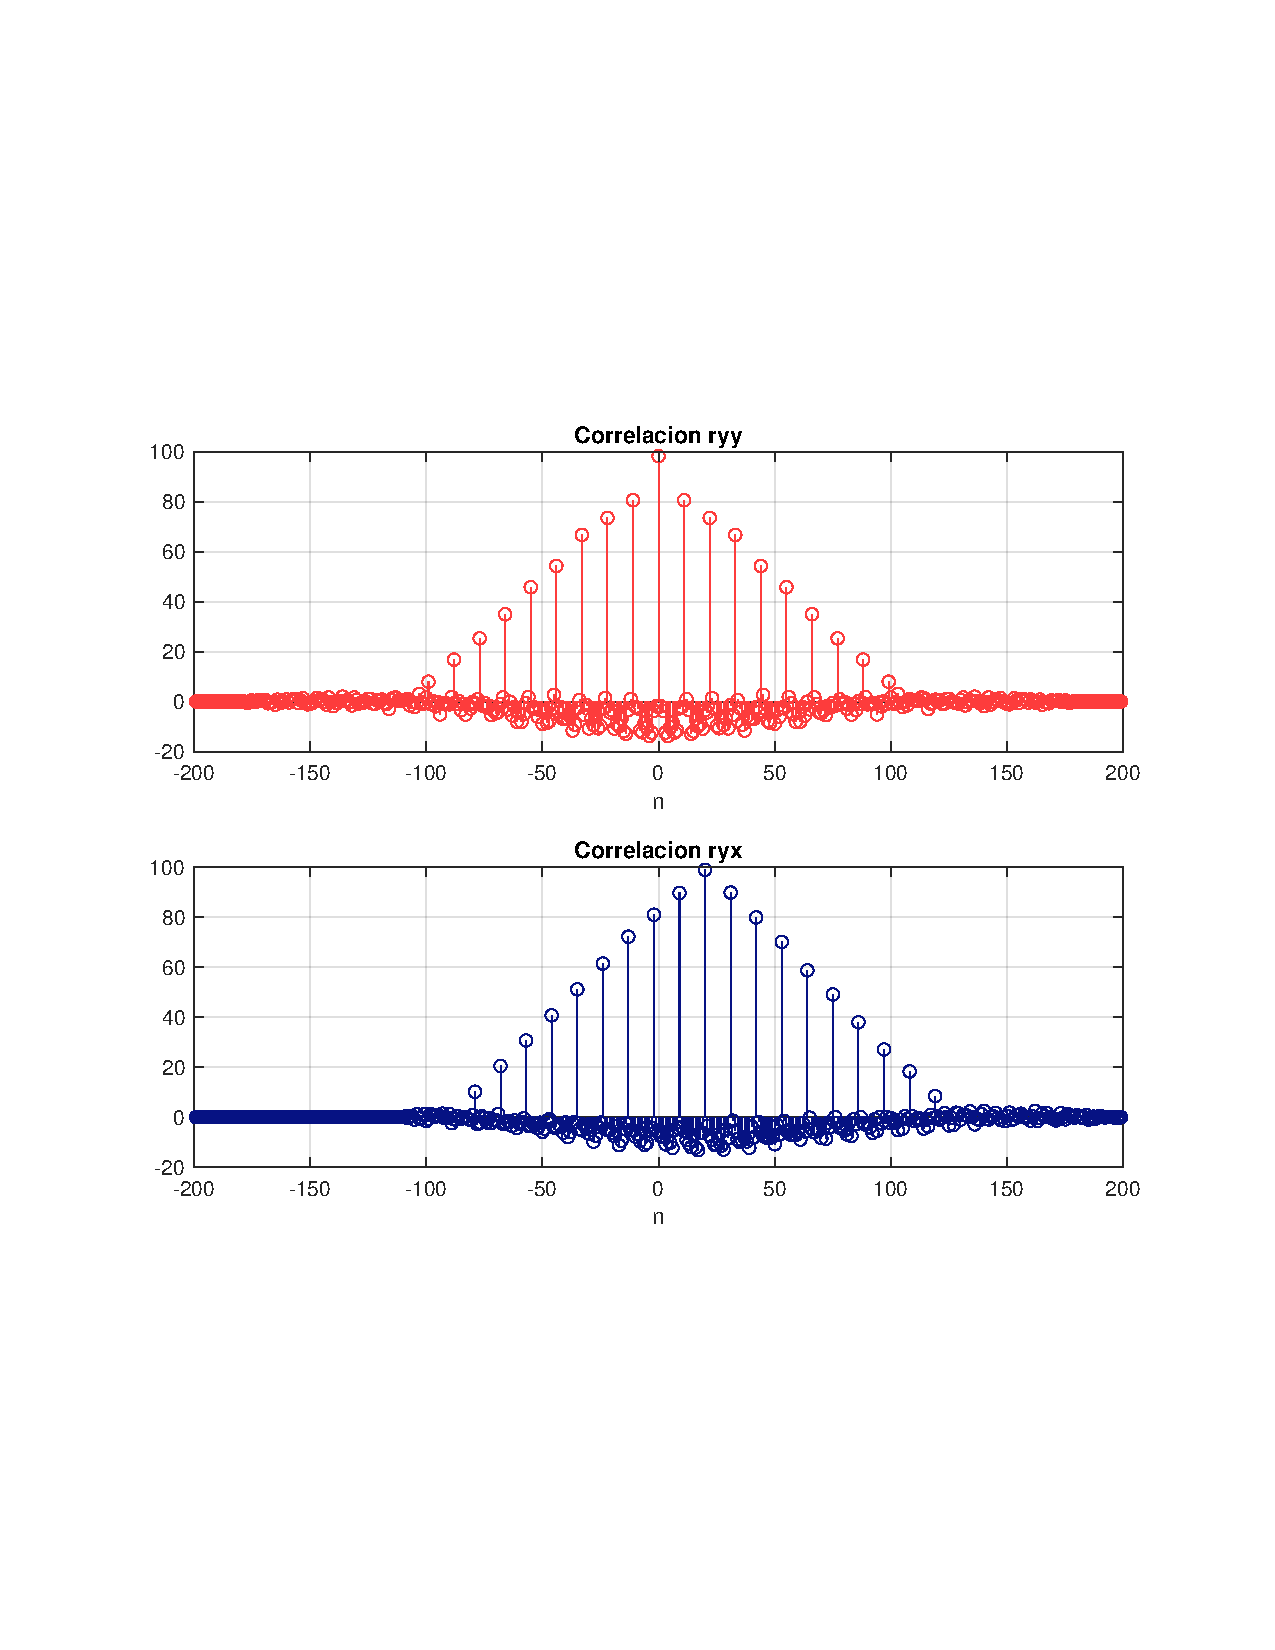
\includegraphics[width=0.6\textwidth,clip, trim = {2cm 7.0cm 2.2cm 7.0cm}]{../imgs/4_radar_e_corre.pdf}
			\caption{Correlación ryy e ryx de la situación anterior}
			\label{fig:radar_e_corre}
		\end{figure}
		
		Note que para esta caso, con diez secuencias de barker continuas, la estimación de D no ha cambiado, se tiene un peak central el cual corresponde al valor esperado, pero ahora es de una \textit{potencia mayor}, también aparecen bandas latearles al peak, que corresponden al desfase temporal entre los pulsos que son enviados. Para este caso, se tiene una mejor resistencia al ruido, teniendo un valor de SNR $\approx$ 10 \textit{dB}.